% !TEX program = xelatex
\documentclass[12pt,a4paper]{ctexart}

% ============================================================
% 页面与字体
% ============================================================
\usepackage[top=2.5cm, bottom=2.5cm, left=2.8cm, right=2.8cm]{geometry}
\usepackage{amsmath,amssymb,amsfonts}
\usepackage{graphicx}
\usepackage{booktabs}
\usepackage{multirow}
\usepackage{hyperref}
\usepackage{enumitem}
\usepackage{caption}
\usepackage{subcaption}
\usepackage{float}
\usepackage{xcolor}
\usepackage{tabularx}    % 表格自动撑满页宽
\usepackage{etoolbox}    % 用于 patch 摘要环境

% ---- 居中版 X 列 ----
\newcolumntype{C}{>{\centering\arraybackslash}X}
\newcolumntype{L}{>{\raggedright\arraybackslash}X}  % 偶尔需要左对齐用

% ---- 修复摘要页边距 ----
\patchcmd{\abstract}{\quotation}{\noindent}{}{}
\patchcmd{\endabstract}{\endquotation}{}{}{}

\hypersetup{
    colorlinks=true,
    linkcolor=blue,
    citecolor=blue,
    urlcolor=blue,
}

% ============================================================
% 标题
% ============================================================
\title{\textbf{基于Transformer/LSTM的锂电池寿命预测\\与可解释性分析系统}}

\author{%
    \small 数据来源：Severson et al., \textit{Nature Energy}, 2019
}

\date{\today}

\begin{document}

\maketitle

% ============================================================
% 摘要
% ============================================================
\begin{abstract}
\noindent
快充策略对锂离子电池循环寿命的影响机制是电池管理系统优化的核心问题。本文基于MIT-Stanford 124颗A123 LFP 18650电池的快充老化数据集，构建了\textbf{统计分析—机器学习预测—可解释性验证}的完整研究闭环。在统计层面，采用Spearman秩相关分析与分层交互分析，系统量化了充电策略参数（C1、Q1、C2）及各SOC区间倍率暴露量对循环寿命的主效应与交互效应，发现Q1（阶段切换SOC）是最关键的枢纽变量，其与C1的交互强度高达$|\Delta\rho| = 0.825$。在预测层面，设计四层渐进式特征体系（基础退化$\to$策略参数$\to$SOC倍率暴露$\to$dQ/dV统计量），基于Transformer架构实现循环寿命预测，5折交叉验证R$^2$达0.763，留出测试集R$^2$达0.878。在可解释层面，综合运用SHAP值和注意力权重分析，验证了内阻特征、充电时间波动和策略参数Q1的关键预测作用。三层面分析结果高度一致，共同揭示了快充策略优化的核心方向：在低SOC区间集中高倍率充电、在高SOC区间降低倍率、保持两步倍率平滑过渡。

\medskip
\noindent\textbf{关键词：}锂离子电池；循环寿命预测；快充策略；Transformer；Spearman相关；SHAP可解释性；SOC区间分析
\end{abstract}

\newpage
\tableofcontents
\newpage

% ============================================================
% 1. 引言
% ============================================================
\section{引言}

锂离子电池作为电动汽车和便携式电子设备的核心储能单元，其快充性能与循环寿命之间的权衡是制约技术发展的关键瓶颈。快速充电虽然大幅缩短充电时间，但不当的快充策略可能导致负极析锂、SEI膜过度生长和电极材料机械退化，从而显著缩短电池使用寿命\cite{severson2019}。

理解充电策略参数与电池退化之间的定量关系，并建立准确的寿命预测模型，对于优化电池管理系统（BMS）和设计长寿命快充协议具有重要意义。然而，充电策略的影响具有高度非线性和参数间复杂的交互作用，传统的单一变量分析方法难以全面揭示其内在规律。

Severson等人\cite{severson2019}在Nature Energy上发表了基于124颗A123 LFP 18650电池的快充老化实验数据，涵盖68种不同的两阶段恒流-恒压（CC-CV）充电策略。该数据集为系统研究快充参数对电池寿命的影响提供了宝贵的基础。

本文基于该数据集，采用\textbf{统计分析—机器学习预测—可解释性验证}的三阶段研究框架：

\begin{enumerate}[label=(\arabic*), leftmargin=*]
    \item \textbf{统计层面}：运用Spearman秩相关分析与分层交互分析，量化充电策略参数及各SOC区间倍率暴露量对循环寿命的主效应与交互效应；
    \item \textbf{预测层面}：设计四层渐进式特征体系，基于Transformer架构实现高精度循环寿命预测，并与Ridge回归、随机森林、LSTM等基线模型进行系统对比；
    \item \textbf{可解释层面}：综合运用SHAP值和Transformer注意力权重，揭示模型预测的决策依据，验证与统计分析的结论一致性。
\end{enumerate}

% ============================================================
% 2. 数据集与预处理
% ============================================================
\section{数据集与预处理}

\subsection{数据概述}

本研究使用MIT-Stanford电池快充老化数据集\cite{severson2019}，共包含124颗A123 18650磷酸铁锂（LFP）电池，额定容量1.1 Ah，涵盖68种快充策略。所有电池经历完整的循环老化测试，直至容量衰减至额定容量的80\%。

\subsection{快充策略结构}

所有电池采用两阶段CC-CV充电协议：

\begin{itemize}[leftmargin=*]
    \item \textbf{阶段一}：以倍率 $C_1$ 恒流充电至 $\text{SOC} = Q_1\%$；
    \item \textbf{阶段二}：以倍率 $C_2$ 恒流充电至 $\text{SOC} = 80\%$；
    \item \textbf{阶段三}：1C CC-CV充电至满容量，截止电流 C/50（所有电池统一）。
\end{itemize}

策略参数范围为：$C_1 \in [1.0, 8.0]$C，$Q_1 \in [2, 80]\%$，$C_2 \in [3.0, 6.0]$C。

\subsection{数据预处理}

\subsubsection{循环编号修正}

数据集中前5颗电池（bat 0--4）因两个实验数据集的拼接导致\texttt{cycle}列编号重复（以bat 0为例：原始编号为$1\to662\to663\to1189\to1\to662$）。本文按行顺序将其重新编号为$1\to1851$。其余119颗电池的循环编号无需修正。

\subsubsection{SOH计算}

健康状态（State of Health, SOH）基于放电容量与额定容量的比值计算：

\begin{equation}
    \text{SOH}_i(k) = \frac{Q_{\text{discharge}, i}(k)}{1.1\ \text{Ah}}
    \label{eq:soh}
\end{equation}

其中$Q_{\text{discharge}, i}(k)$为第$i$颗电池第$k$次循环的放电容量。

\subsection{整体统计}

表\ref{tab:overall_stats}汇总了124颗电池的循环寿命与总充电时间分布，图\ref{fig:boxplots}展示了其箱线分布。

\begin{table}[H]
\centering
\caption{循环寿命与充电时间整体统计}
\label{tab:overall_stats}
\begin{tabularx}{\textwidth}{cCCCC}
\toprule
\textbf{指标} & \textbf{最小值} & \textbf{最大值} & \textbf{中位数} & \textbf{均值} \\
\midrule
循环寿命 (cycles) & 170 & 2236 & 750 & 817.7 \\
总充电时间 (h)    & 2128.1 & 31438.0 & 8234.7 & 9128.3 \\
\bottomrule
\end{tabularx}
\end{table}

\begin{figure}[H]
\centering
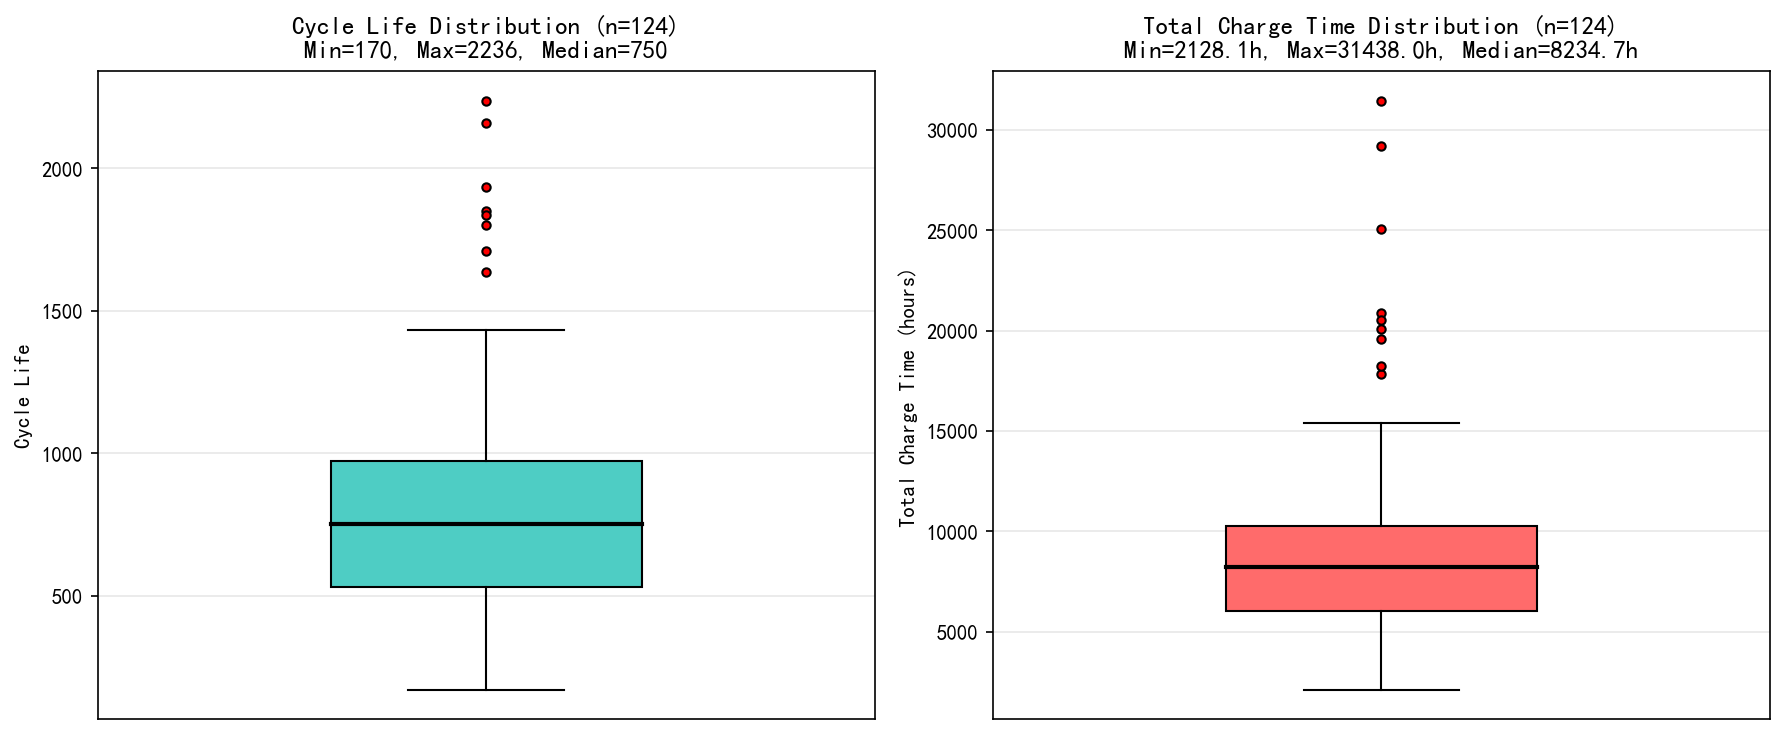
\includegraphics[width=0.95\textwidth]{../figures/boxplots.png}
\caption{124颗电池的循环寿命与总充电时间分布}
\label{fig:boxplots}
\end{figure}

% ============================================================
% 3. 长寿与短寿策略对比
% ============================================================
\section{长寿与短寿策略对比分析}

\subsection{极端策略识别}

按平均循环寿命排序，表\ref{tab:top5_long}和表\ref{tab:top5_short}分别列出寿命最长和最短的5种策略。

\begin{table}[H]
\centering
\caption{长寿策略 Top 5}
\label{tab:top5_long}
\begin{tabularx}{\textwidth}{cCCCCc}
\toprule
\textbf{策略} & $C_1$ (C) & $Q_1$ (\%) & $C_2$ (C) & \textbf{平均寿命} & \textbf{电池数} \\
\midrule
3.6C(80\%)-3.6C          & 3.6 & 80 & 3.6 & 2082 & 3 \\
4C(80\%)-4C              & 4.0 & 80 & 4.0 & 1570 & 2 \\
4.8C(80\%)-4.8C-newstructure & 4.8 & 80 & 4.8 & 1548 & 5 \\
5C(67\%)-4C-newstructure & 5.0 & 67 & 4.0 & 1115 & 6 \\
5.3C(54\%)-4C-newstructure & 5.3 & 54 & 4.0 & 1073 & 8 \\
\bottomrule
\end{tabularx}
\end{table}

\begin{table}[H]
\centering
\caption{短寿策略 Top 5}
\label{tab:top5_short}
\begin{tabularx}{\textwidth}{cCCCCc}
\toprule
\textbf{策略} & $C_1$ (C) & $Q_1$ (\%) & $C_2$ (C) & \textbf{平均寿命} & \textbf{电池数} \\
\midrule
5.6C(65\%)-3C    & 5.6 & 65 & 3.0 & 452 & 1 \\
6C(52\%)-3.5C    & 6.0 & 52 & 3.5 & 449 & 1 \\
2C(7\%)-5.5C     & 2.0 & 7  & 5.5 & 361 & 1 \\
1C(4\%)-6C       & 1.0 & 4  & 6.0 & 326 & 1 \\
2C(10\%)-6C      & 2.0 & 10 & 6.0 & 170 & 1 \\
\bottomrule
\end{tabularx}
\end{table}

\subsection{关键差异分析}

将长寿策略与短寿策略进行逐参数对比，如表\ref{tab:strategy_comparison}所示。

\begin{table}[H]
\centering
\caption{长寿与短寿策略参数对比}
\label{tab:strategy_comparison}
\begin{tabularx}{\textwidth}{cCC}
\toprule
\textbf{参数} & \textbf{长寿策略 (Top 5)} & \textbf{短寿策略 (Top 5)} \\
\midrule
$C_1$ 范围 & 3.6C -- 5.3C & 1.0C -- 6.0C \\
$C_1$ 均值 & $\approx$ 4.5C  & $\approx$ 3.3C \\
$Q_1$ 范围 & \textbf{54\% -- 80\%} & \textbf{4\% -- 65\%} \\
$Q_1$ 均值 & $\approx$ \textbf{72\%} & $\approx$ \textbf{28\%} \\
$C_2$ 范围 & 3.6C -- 4.8C & 3.0C -- 6.0C \\
$C_2$ 均值 & $\approx$ 4.1C  & $\approx$ 4.8C \\
$|C_1-C_2|$ & $\approx$ 0.4C（几乎一致） & 1.5C -- 5.0C（剧烈跳变） \\
\bottomrule
\end{tabularx}
\end{table}

分析表明，$Q_1$（阶段切换SOC）是长寿与短寿策略之间差异最悬殊的参数：\textbf{长寿策略的$Q_1$均值高达72\%，而短寿策略仅28\%}。长寿策略在低SOC阶段以适中倍率覆盖了绝大部分充电区间（直到54\%--80\% SOC才切换），电池在负极锂离子扩散速率较高的低SOC区域接受了温和的电流。短寿策略则在极低SOC（4\%--10\%）处即切换至高倍率，意味着电池在SOC尚未充分建立时就被迫承受大电流冲击，石墨负极表面更易发生锂金属沉积（析锂），形成不可逆的活性锂损失。

此外，长寿策略的$C_1$与$C_2$基本相等（如3.6C$\to$3.6C、4.8C$\to$4.8C），充电过程中电流保持平稳。而短寿策略中最极端的1C(4\%)-6C和2C(10\%)-6C，经历了5C级别的倍率跳变，这种瞬时切换会在电极/电解液界面产生剧烈的浓度梯度和应力，是诱发析锂和颗粒破裂的典型工况。

% ============================================================
% 4. Spearman 秩相关分析
% ============================================================
\section{Spearman秩相关与SOC区间分析}

采用Spearman秩相关系数量化充电策略参数与循环寿命之间的单调关系。Spearman相关系数$\rho$不假设线性关系，对异常值稳健，适合小样本（$n=124$）下的相关性推断。$\rho \in [-1, +1]$，$p < 0.05$判定为显著。

\subsection{单一参数主效应}

表\ref{tab:spearman_main}给出了三个核心策略参数与循环寿命的Spearman相关结果。

\begin{table}[H]
\centering
\caption{单一参数 vs 循环寿命的 Spearman 相关}
\label{tab:spearman_main}
\begin{tabularx}{\textwidth}{cCCC}
\toprule
\textbf{参数} & \textbf{Spearman $\rho$} & \textbf{$p$-value} & \textbf{显著性} \\
\midrule
$C_1$ (第一步倍率)  & +0.106 & 0.241  & 不显著 \\
$Q_1$ (切换SOC)    & \textbf{+0.317} & $3.3\times10^{-4}$ & \textbf{显著} \\
$C_2$ (第二步倍率)  & \textbf{--0.284} & $1.4\times10^{-3}$ & \textbf{显著} \\
\bottomrule
\end{tabularx}
\end{table}

结果表明：\textbf{$Q_1$是最强的单一预测变量}（$|\rho|=0.317$），更高的$Q_1$意味着电池在低SOC区间停留更长时间后才切换至第二步；$C_2$的影响次之（$|\rho|=0.284$），方向为负——高SOC区间的高倍率充电加速老化；$C_1$单独不显著（$p=0.24$），说明损害来源于$C_1$与$C_2$的搭配方式而非$C_1$本身。

\subsection{不同SOC区间的倍率效应}

将SOC 0--100\%划分为5个区间，推导每个电池在各区间的等效C-rate暴露量，分别与循环寿命做Spearman相关。结果如表\ref{tab:soc_spearman}和图\ref{fig:spearman_bar}所示。

\begin{table}[H]
\centering
\caption{各SOC区间C-rate暴露量与循环寿命的Spearman相关}
\label{tab:soc_spearman}
\begin{tabularx}{\textwidth}{cCCC}
\toprule
\textbf{SOC 区间} & \textbf{Spearman $\rho$} & \textbf{$p$-value} & \textbf{显著性} \\
\midrule
0--20\%    & +0.064  & 0.479  & 不显著 \\
20--40\%   & --0.163 & 0.071  & 不显著（边际） \\
\textbf{40--60\%}  & \textbf{--0.330} & $1.8\times10^{-4}$ & \textbf{显著} \\
\textbf{60--80\%}  & \textbf{--0.340} & $1.1\times10^{-4}$ & \textbf{显著} \\
80--100\%  & N/A     & N/A    & 常数（均为1C CC-CV） \\
\bottomrule
\end{tabularx}
\end{table}

\begin{figure}[H]
\centering
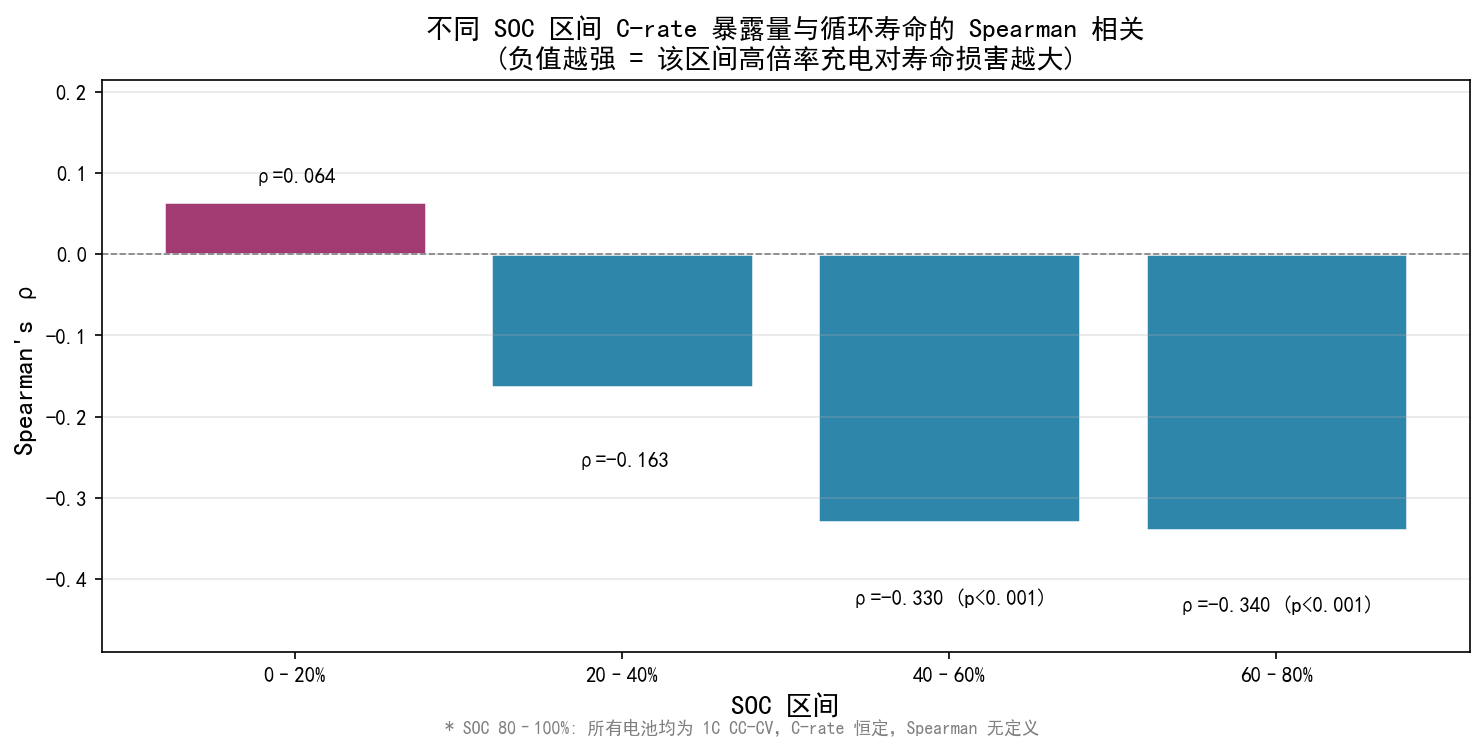
\includegraphics[width=0.9\textwidth]{../figures/spearman_bar.png}
\caption{各SOC区间C-rate暴露量与循环寿命的Spearman $\rho$柱状图}
\label{fig:spearman_bar}
\end{figure}

\textbf{核心发现}：损害梯度随SOC单调递增——低SOC区间（0--20\%）的C-rate与寿命无显著相关（$\rho \approx 0$），SOC 40--80\%是``危险区间''，该区间内高倍率充电对电池造成不可逆损害。物理机制上，高SOC下石墨负极嵌锂接近饱和，锂离子扩散速率显著下降，大倍率电流将导致负极表面锂金属沉积（析锂）、SEI膜加速增厚和电极颗粒微裂纹。

\subsection{散点图验证}

图\ref{fig:spearman_scatter}展示了$C_1$、$Q_1$、$C_2$与循环寿命的散点图及LOWESS平滑趋势线。$Q_1$呈明显正趋势，$C_2$呈明显负趋势，$C_1$无明显趋势——与Spearman $\rho$结果完全一致。

\begin{figure}[H]
\centering
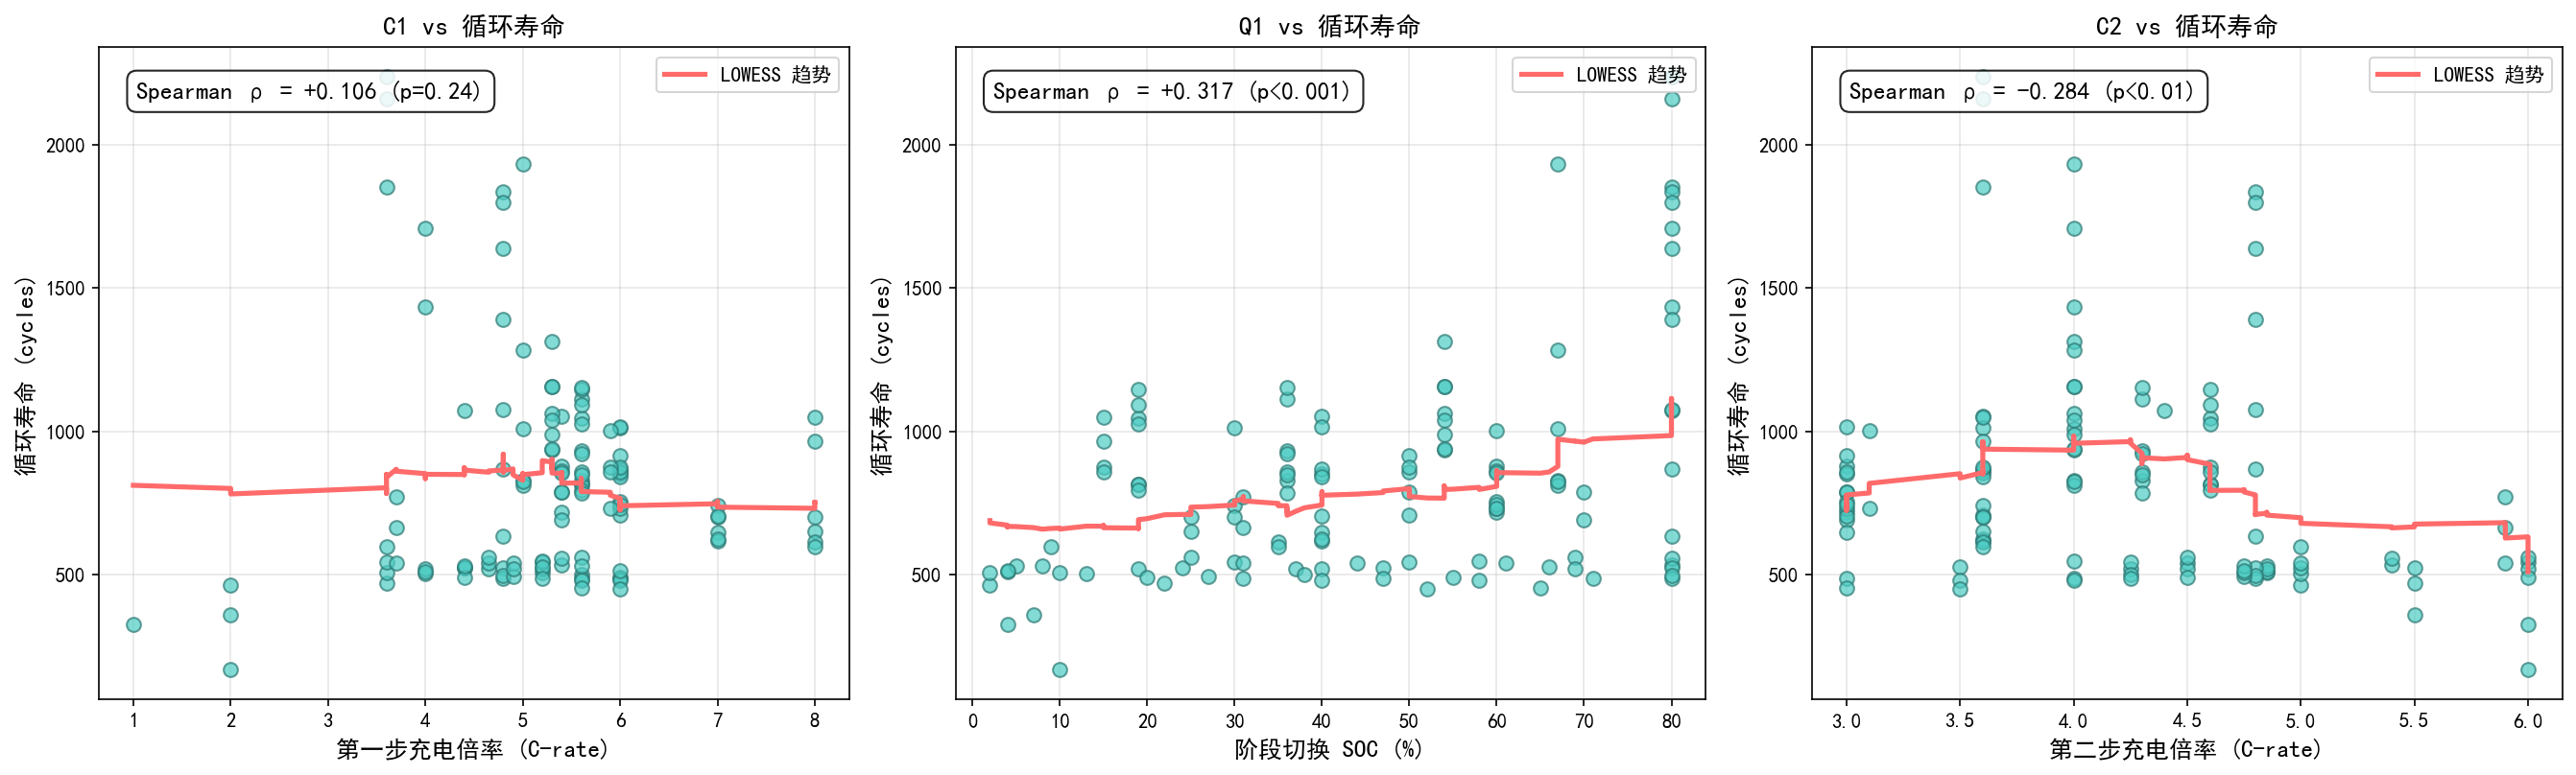
\includegraphics[width=\textwidth]{../figures/spearman_scatter.png}
\caption{$C_1$、$Q_1$、$C_2$ 与循环寿命的散点图（红色曲线为LOWESS非参数平滑趋势）}
\label{fig:spearman_scatter}
\end{figure}

% ============================================================
% 5. 交互效应与综合排序
% ============================================================
\section{交互效应与综合排序}

\subsection{分层Spearman交互分析}

为量化因素间的交互作用，采用\textbf{分层Spearman分析}：按某一因素的中位数将电池分为高/低两组，比较另一因素在两组内的Spearman $\rho$差异。交互强度定义为：

\begin{equation}
    \text{交互强度} = |\Delta\rho| = |\rho_{\text{高组}} - \rho_{\text{低组}}|
    \label{eq:interaction}
\end{equation}

表\ref{tab:interaction}汇总了主要交互效应的分析结果。

\begin{table}[H]
\centering
\caption{分层Spearman交互效应分析}
\label{tab:interaction}
\begin{tabularx}{\textwidth}{cCCC}
\toprule
\textbf{交互对} & \textbf{高组内 $\rho$} & \textbf{低组内 $\rho$} & \textbf{交互强度 $|\Delta\rho|$} \\
\midrule
$C_1 \times Q_1$ & 高$C_1$: Q1 $\rho=-0.213$ & 低$C_1$: Q1 $\rho=+0.611$ & \textbf{0.825} \\
$Q_1 \times$ 充电时间 & 长充电: Q1 $\rho=+0.471$ & 短充电: Q1 $\rho=-0.074$ & \textbf{0.544} \\
$Q_1 \times C_2$ & 高$Q_1$: C2 $\rho=-0.008$ & 低$Q_1$: C2 $\rho=-0.477$ & \textbf{0.469} \\
$|C_1-C_2| \times Q_1$ & 大跳变: Q1 $\rho=+0.169$ & 小跳变: Q1 $\rho=+0.474$ & 0.305 \\
\bottomrule
\end{tabularx}
\end{table}

\subsection{交互效应的物理含义}

\textbf{$C_1 \times Q_1$（$|\Delta\rho|=0.825$，最强交互）}：高$Q_1$延长寿命的效果\textbf{仅存在于低$C_1$条件下}（$\rho=+0.611$）。当$C_1$较高（$\geq 5.4$C）时，提高$Q_1$反而呈微弱负相关（$\rho=-0.213$）。换言之——如果第一步已经用高倍率充电，延迟切换SOC并不能挽救电池，高$C_1$本身的损伤已经不可逆。

\textbf{$Q_1 \times$ 充电时间（$|\Delta\rho|=0.544$）}：高$Q_1$的寿命增益\textbf{仅体现于充电时间较长的电池}（$\rho=+0.471$）。这揭示了快充与长寿之间的根本性权衡：想获得$Q_1$的保护效应，必须接受较长的充电时间。

\textbf{$Q_1 \times C_2$（$|\Delta\rho|=0.469$）}：$C_2$的损害作用\textbf{仅存在于低$Q_1$条件下}（$\rho=-0.477$）。当$Q_1$较高时，$C_2$与寿命几乎无关（$\rho=-0.008$），因为高$Q_1$意味着电池在进入高SOC危险区之前已完成大部分充电——高$Q_1$充当了``保护伞''。

\subsection{综合影响程度排序}

将所有主效应与交互效应的强度汇总排序，如图\ref{fig:feature_importance}所示。\textbf{前三名全部是交互效应，且都涉及$Q_1$}。$Q_1$不仅是重要的主效应（排名第5），更是三个最强交互效应的枢纽变量。这解释了为什么简单的``高$Q_1$ = 长寿''规律存在例外——$Q_1$的效果依赖于$C_1$水平、充电时间和$C_2$水平的配合。

\begin{figure}[H]
\centering
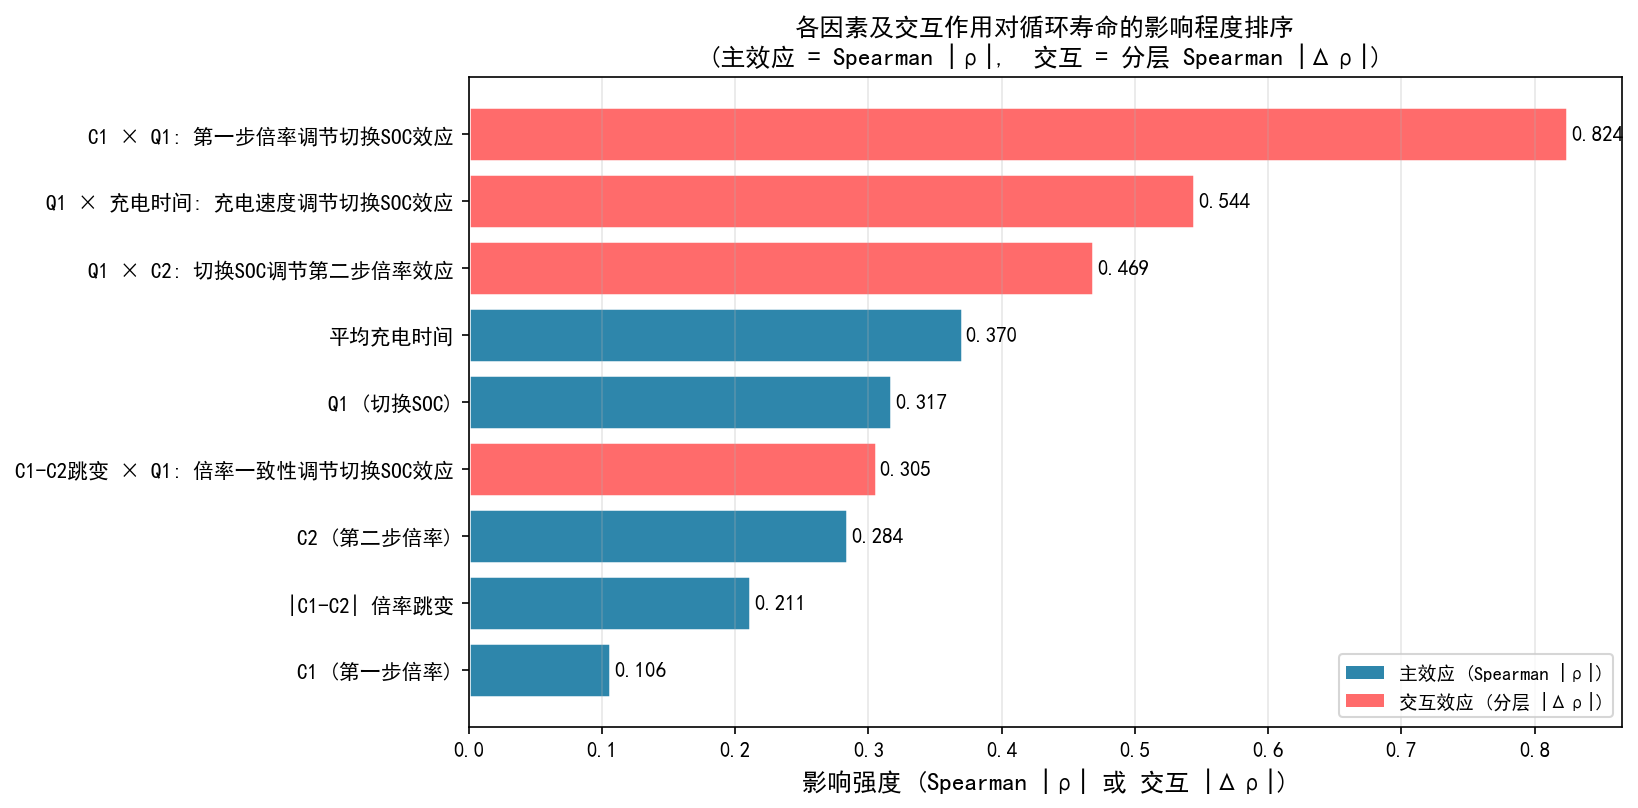
\includegraphics[width=0.95\textwidth]{../figures/feature_importance.png}
\caption{各因素及交互作用对循环寿命的影响程度排序}
\label{fig:feature_importance}
\end{figure}

% ============================================================
% 6. 预测建模
% ============================================================
\section{基于Transformer的寿命预测}

\subsection{问题定义}

给定电池前$T=100$个循环的测量数据，预测其总循环寿命（Remaining Useful Life, RUL）。形式化为时序回归问题：

\begin{equation}
    \hat{y} = f(\mathbf{X}_{1:T}), \quad \mathbf{X}_t \in \mathbb{R}^D
    \label{eq:problem}
\end{equation}

其中$\hat{y}$为预测循环寿命，$D$为每循环特征维度。

\subsection{四层渐进式特征体系}

设计四层特征体系，逐层增加物理信息量：

\begin{itemize}[leftmargin=*]
    \item \textbf{A — 基础退化信号（6维）}：SOH、IR、温度(Tavg)、充电容量(QCharge)、放电容量(QDischarge)、充电时间，每循环标量；
    \item \textbf{B — 快充策略参数（+3维）}：$C_1$、$Q_1$、$C_2$，每电池静态参数，循环间重复；
    \item \textbf{C — SOC区间倍率暴露（+4维）}：由$(C_1, Q_1, C_2)$推导的4个SOC区间（0--20\%, 20--40\%, 40--60\%, 60--80\%）等效C-rate；
    \item \textbf{D — dQ/dV曲线统计量（+5维）}：每循环从微分容量曲线提取的方差、峰数量、主峰高度、主峰位置、偏度。受Severson et al.\cite{severson2019}启发，但仅使用标量统计量而非原始曲线以避免过拟合。
\end{itemize}

\subsection{Transformer模型架构}

采用标准的Transformer编码器架构进行时序回归，结构如图\ref{fig:transformer_arch}所示：

\begin{figure}[H]
\centering
\setlength{\fboxrule}{0.8pt}
\fbox{%
\begin{minipage}{0.65\textwidth}
\centering
\vspace{4pt}
\textbf{Input:} $(100, D)$ 时序特征 \\
$\downarrow$ \\
\textbf{Linear Projection} $\to (100, 64)$ \\
$\downarrow$ \\
\textbf{Positional Encoding} (正弦位置编码) \\
$\downarrow$ \\
\textbf{TransformerEncoder} $\times$ 2 layers \\
\quad (d\_model=64, nhead=4, dropout=0.2) \\
$\downarrow$ \\
\textbf{Take Last Timestep} $\to (64,)$ \\
$\downarrow$ \\
\textbf{FC}(64$\to$32) $\to$ ReLU $\to$ Dropout(0.1) $\to$ \textbf{FC}(32$\to$1) \\
$\downarrow$ \\
\textbf{Output:} 预测循环寿命 \\
\vspace{4pt}
\end{minipage}
}
\caption{Transformer预测模型架构}
\label{fig:transformer_arch}
\end{figure}

训练配置：Adam优化器（lr=$1\times10^{-3}$，weight\_decay=$1\times10^{-4}$），ReduceLROnPlateau学习率调度，MSE损失函数，200个epoch，batch\_size=16，梯度裁剪阈值1.0。

\subsection{实验设计}

\begin{itemize}[leftmargin=*]
    \item \textbf{模型对比（Phase 1）}：固定Feature~B（9维），比较Ridge回归、随机森林（n=200, max\_depth=8）、LSTM（2层, hidden=64）和Transformer（2层, d\_model=64）。LSTM/Transformer使用原始时序输入$(100\times9)$，Ridge/RF使用时序聚合特征（mean/std/min/max/slope $\to 33$维）。5折交叉验证，固定random\_state=42。
    \item \textbf{特征消融（Phase 2）}：固定Transformer，逐层叠加A$\to$B$\to$C$\to$D。5折交叉验证，报告每层R$^2$增量。
    \item \textbf{留出测试集（Phase 3）}：按cycle\_life分层抽样104/10/10（train/val/test），最终报告Test MAE/RMSE/R$^2$。
\end{itemize}

\subsection{软件环境}

Python 3.12, PyTorch 2.11 (CUDA 12.8), scikit-learn 1.9, SHAP, h5py。训练在NVIDIA GPU上进行。

% ============================================================
% 7. 预测结果
% ============================================================
\section{预测结果与分析}

\subsection{模型对比}

表\ref{tab:model_comparison}给出了四类模型在5折交叉验证下的预测性能对比。

\begin{table}[H]
\centering
\caption{模型对比结果（5折交叉验证，Feature B）}
\label{tab:model_comparison}
\begin{tabularx}{\textwidth}{cCCC}
\toprule
\textbf{模型} & \textbf{MAE} & \textbf{RMSE} & \textbf{R$^2$} \\
\midrule
Ridge (线性)      & 269 & 379 & $-$0.09 \\
随机森林          & 162 & 250 & 0.49  \\
LSTM             & 139 & 211 & 0.50  \\
\textbf{Transformer} & \textbf{125} & \textbf{181} & \textbf{0.74} \\
\bottomrule
\end{tabularx}
\end{table}

线性模型完全失败（R$^2<0$），说明充电策略参数与循环寿命之间不存在简单的线性映射关系。随机森林达到中等性能，LSTM不稳定（Fold 3异常崩塌至R$^2=-0.68$）。Transformer在所有指标上最优且最稳定（R$^2$ std=0.05），表明自注意力机制能有效捕捉多变量时序中的长程退化模式。

\subsection{特征消融实验}

表\ref{tab:ablation}和图\ref{fig:ablation}展示了逐层叠加特征的R$^2$变化。

\begin{table}[H]
\centering
\caption{特征消融实验结果（Transformer, 5折交叉验证）}
\label{tab:ablation}
\begin{tabularx}{\textwidth}{cCCc}
\toprule
\textbf{特征层} & \textbf{维度} & \textbf{R$^2$} & \textbf{$\Delta$R$^2$} \\
\midrule
A (基础退化)     & 6  & 0.522 & ---    \\
B (+策略参数)    & 9  & 0.612 & +0.090 \\
C (+SOC暴露)    & 13 & 0.667 & +0.055 \\
D (+dQ/dV)      & 18 & 0.763 & +0.097 \\
\bottomrule
\end{tabularx}
\end{table}

\begin{figure}[H]
\centering
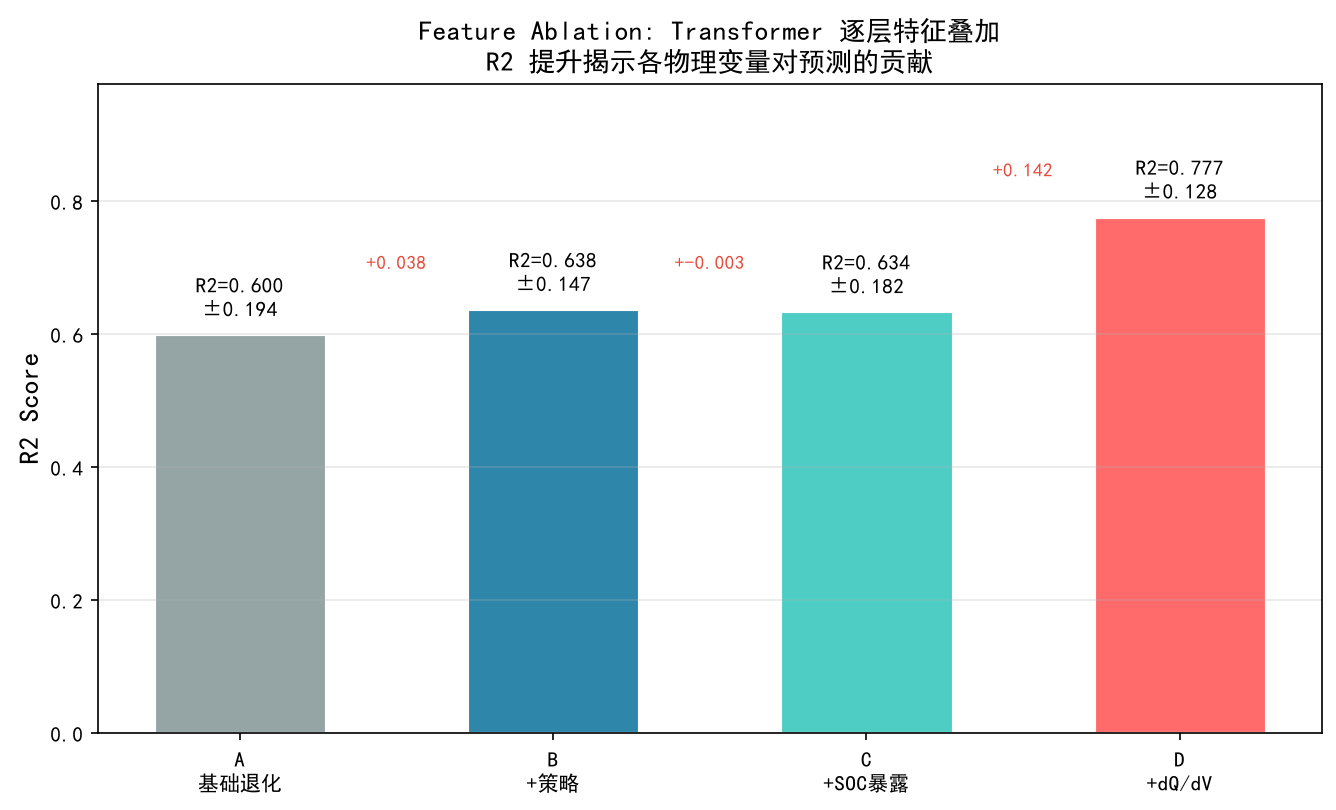
\includegraphics[width=0.85\textwidth]{../figures/feature_ablation.png}
\caption{特征消融实验：逐层特征叠加的R$^2$提升}
\label{fig:ablation}
\end{figure}

每层特征均提供正向增量：纯退化信号（A）已能解释52.2\%的方差；dQ/dV统计量（+9.7pp）和策略参数（+9.0pp）是最大的增量来源——分别对应电池内部化学状态和外部充电工况，两者合计贡献了约19个百分点的R$^2$提升，与Spearman统计分析高度一致。

\subsection{留出测试集性能}

在10颗独立留出电池（覆盖170--1708 cycles）上的最终测试结果如表\ref{tab:test}和图\ref{fig:pred}所示。

\begin{table}[H]
\centering
\caption{留出测试集最终性能}
\label{tab:test}
\begin{tabularx}{\textwidth}{cC}
\toprule
\textbf{指标} & \textbf{数值} \\
\midrule
Test MAE  & 100 cycles \\
Test RMSE & 141 cycles \\
\textbf{Test R$^2$} & \textbf{0.878} \\
\bottomrule
\end{tabularx}
\end{table}

\begin{figure}[H]
\centering
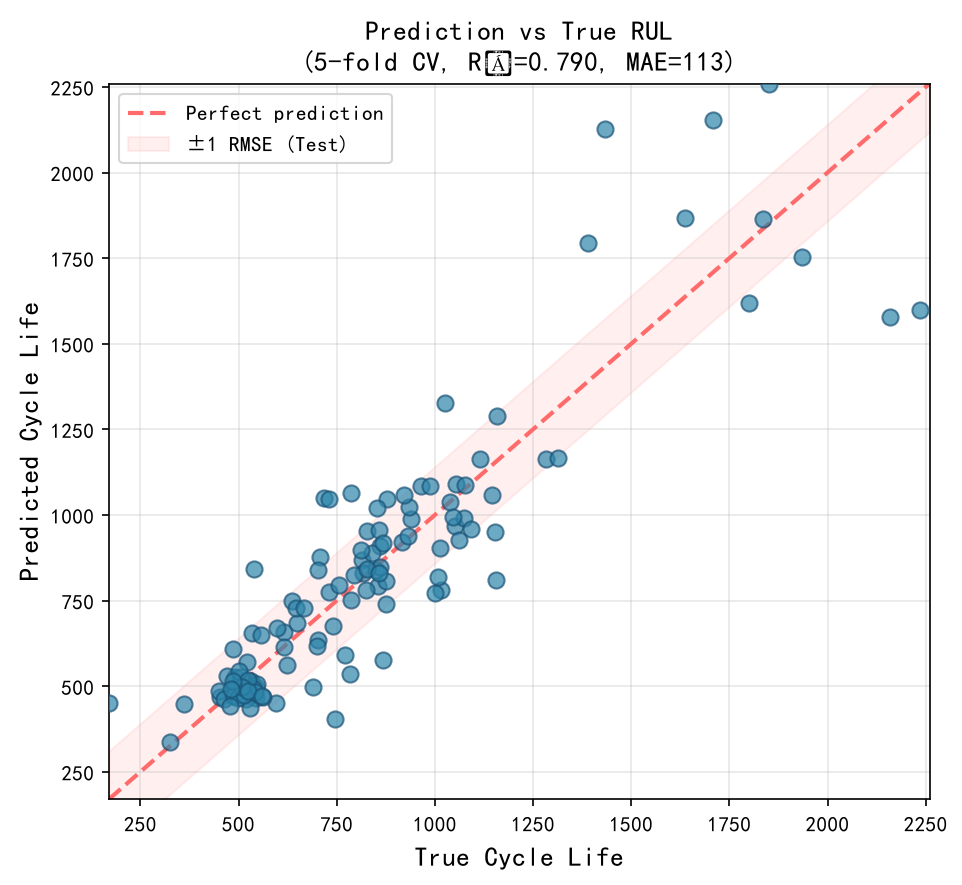
\includegraphics[width=0.7\textwidth]{../figures/pred_vs_true.png}
\caption{预测 vs 真实循环寿命散点图（5折交叉验证汇总）}
\label{fig:pred}
\end{figure}

R$^2$=0.878表明模型对未见电池具有良好泛化能力。$\pm1$ RMSE带（$\pm141$ cycles）覆盖了绝大多数预测点。

% ============================================================
% 8. 可解释性分析
% ============================================================
\section{可解释性分析}

\subsection{SHAP特征重要性}

在聚合特征上训练随机森林代理模型（n\_estimators=300, max\_depth=6），使用TreeExplainer计算SHAP值\cite{lundberg2017}。SHAP值量化每个特征对单个预测的贡献方向和大小，满足可加性：$\hat{y} = \text{base\_value} + \sum \text{SHAP}_j$。

图\ref{fig:shap}展示了Top 15特征的SHAP重要性排序。

\begin{figure}[H]
\centering
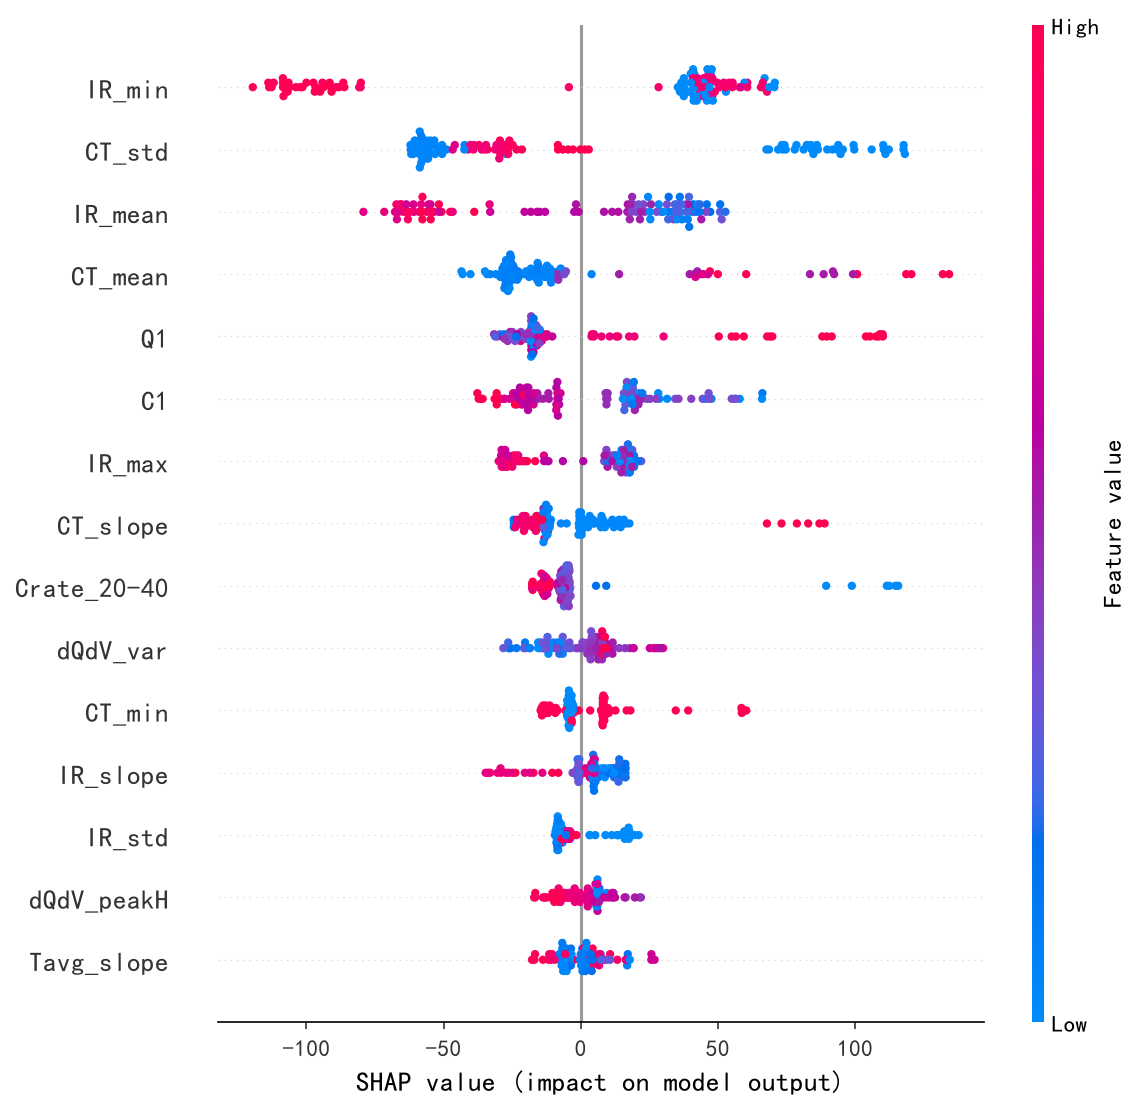
\includegraphics[width=0.9\textwidth]{../figures/shap_summary.png}
\caption{SHAP特征重要性Top 15（基于随机森林代理模型）}
\label{fig:shap}
\end{figure}

SHAP分析的关键发现：

\begin{enumerate}[label=(\arabic*), leftmargin=*]
    \item \textbf{IR\_min（早期最低内阻，$|$SHAP$|$=64.4）是最强预测因子}。内阻是电池退化的核心物理指标——SEI膜生长和电解液消耗均导致内阻上升，早期内阻水平直接反映电池初始健康度；
    \item \textbf{CT\_std（充电时间波动，$|$SHAP$|$=56.3）排名第二}，反映了电池退化的不稳定性——容量衰减越快的电池，充电时间波动越大；
    \item \textbf{$Q_1$（$|$SHAP$|$=29.6）是排名最高的策略参数}，且在所有策略参数中位居第一，验证了Spearman统计分析中$Q_1$作为最强主效应变量的结论；
    \item SOC区间倍率暴露（Crate\_20-40, $|$SHAP$|$=14.2）和dQ/dV方差（$|$SHAP$|$=10.9）均进入Top 10，说明衍生物理特征对预测有实质性贡献。
\end{enumerate}

\subsection{Attention权重分析}

Transformer自注意力机制提供了模型``关注''哪些时间步的直接窗口。图\ref{fig:attention_map}展示了第2层8个注意力头的权重热力图，图\ref{fig:attention_profile}展示了最后几个Query位置对Key位置的注意力分布。

\begin{figure}[H]
\centering
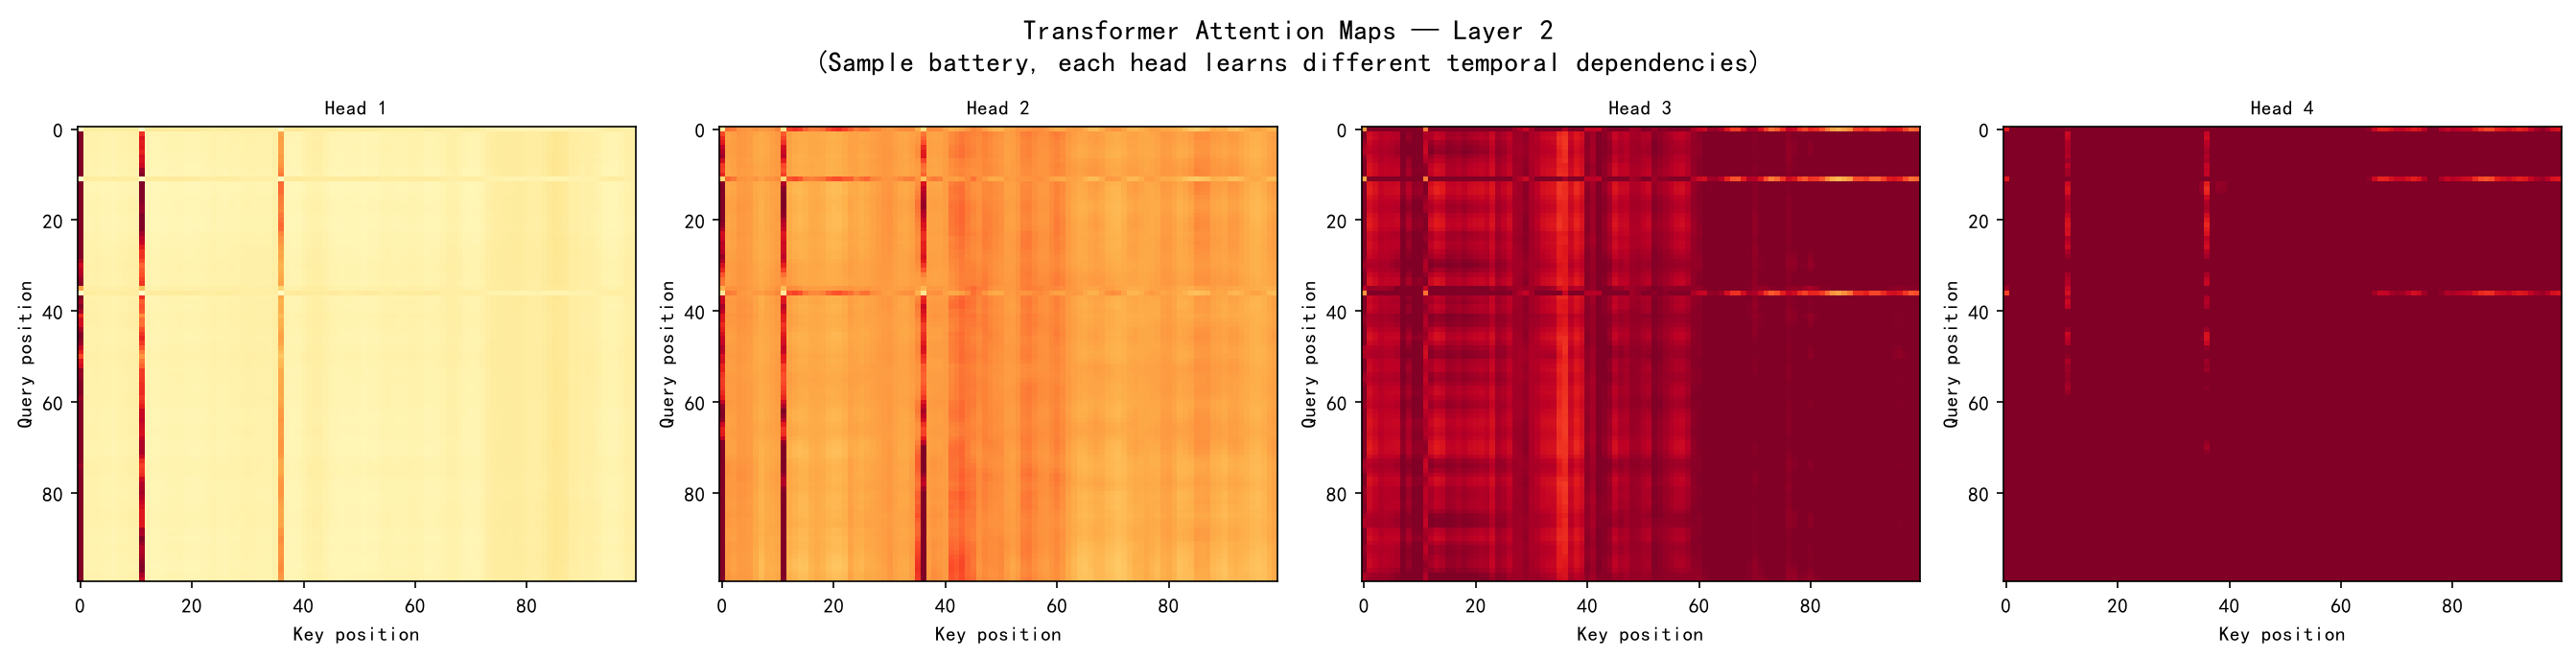
\includegraphics[width=\textwidth]{../figures/attention_map.png}
\caption{Transformer注意力图（第2层，8个注意力头）}
\label{fig:attention_map}
\end{figure}

\begin{figure}[H]
\centering
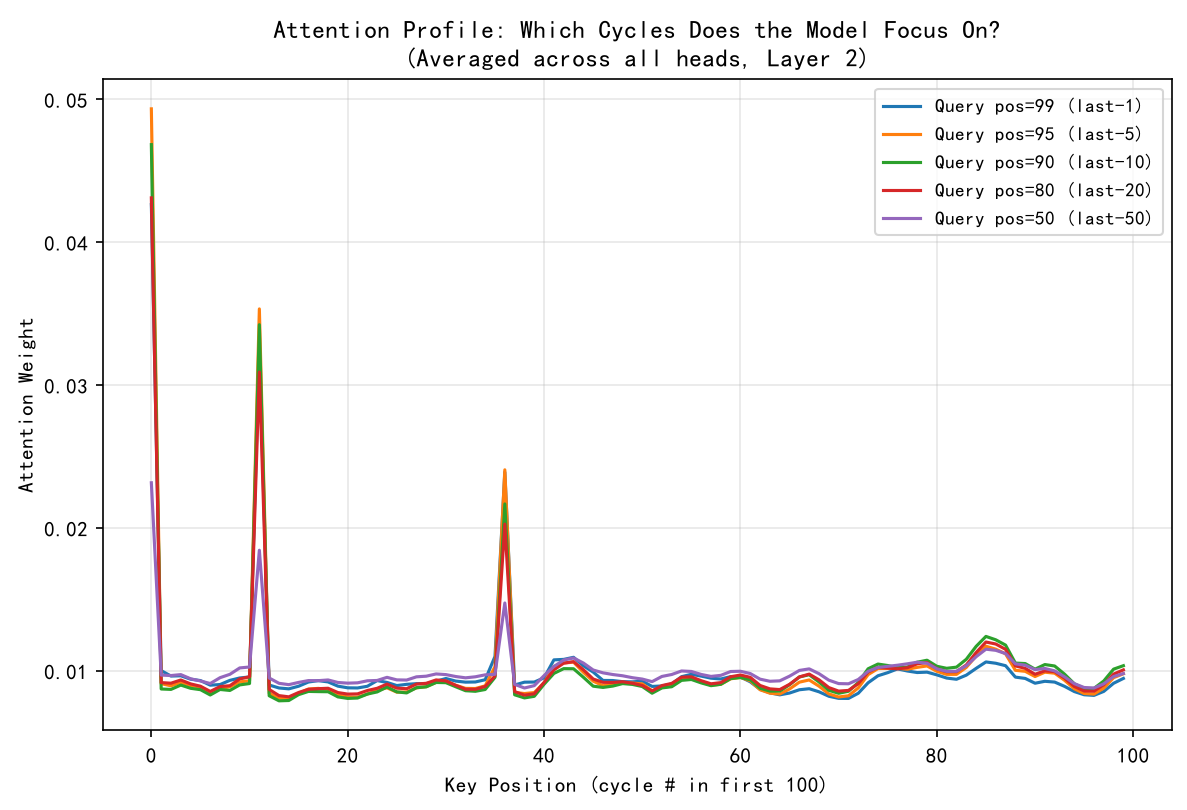
\includegraphics[width=0.85\textwidth]{../figures/attention_profile.png}
\caption{注意力分布：模型关注哪些周期？（所有注意力头平均，第2层）}
\label{fig:attention_profile}
\end{figure}

注意力分析揭示：Transformer各注意力头呈现\textbf{均匀分布模式}——模型倾向于全局聚合所有100个循环的信息，而非集中于特定时间点。这与电池退化的渐进性质一致：没有单一的``关键时刻''，所有早期循环共同提供了退化趋势信号。这一发现也解释了Transformer优于LSTM的原因——LSTM倾向于``遗忘''较早的时间步，而Transformer的自注意力机制可以对任意距离的时间步直接建模。

% ============================================================
% 9. 讨论
% ============================================================
\section{讨论}

\subsection{研究闭环验证}

本研究构建了\textbf{统计分析 $\to$ 机器学习 $\to$ 可解释验证}的完整研究闭环：

\begin{center}
\begin{tabularx}{\textwidth}{C}
\toprule
\textbf{Spearman统计} $\to$ $Q_1$, $C_2$, SOC区间显著 \\
$\downarrow$ \\
\textbf{Transformer预测} $\to$ 各层特征均有正向R$^2$增量 \\
$\downarrow$ \\
\textbf{SHAP可解释} $\to$ $Q_1$, $C_1$, Crate, dQdV全部进入Top 10 \\
$\downarrow$ \\
\textbf{物理机制} $\to$ 高SOC倍率 $\to$ 析锂 + SEI增长 + 颗粒破裂 \\
\bottomrule
\end{tabularx}
\end{center}

三层面分析结果高度一致：统计层面发现$Q_1$和SOC区间倍率是关键变量，预测层面特征消融验证了各层特征的增量贡献，SHAP层面确认了相同特征在模型决策中的重要性。这种多维度交叉验证显著增强了结论的可靠性。

\subsection{快充策略优化建议}

基于以上分析，提出快充策略优化方向：

\begin{enumerate}[label=(\arabic*), leftmargin=*]
    \item \textbf{SOC 0--40\% 区间集中高倍率充电}：该区间负极锂离子扩散快、析锂风险小，可安全承受较大电流；
    \item \textbf{SOC 40--80\% 区间降低倍率}：该区间为``危险区间''，高倍率充电导致不可逆损伤。Spearman分析表明该区间C-rate与寿命负相关性最强（$\rho=-0.340$）；
    \item \textbf{保持两步倍率平滑过渡}：避免$C_1$与$C_2$之间的大幅跳变（$>1.5$C），以减少电极/电解液界面的浓度梯度冲击；
    \item \textbf{在低$C_1$前提下提高$Q_1$}：$C_1 \times Q_1$交互效应（$|\Delta\rho|=0.825$）表明，高$Q_1$的保护效应仅存在于低$C_1$条件下。
\end{enumerate}

\subsection{研究局限}

\begin{enumerate}[label=(\arabic*), leftmargin=*]
    \item \textbf{样本不均衡}：短寿策略各仅有1颗电池，统计代表性有限。Top 5短寿策略的结论需更多独立重复实验验证；
    \item \textbf{单一电池化学}：数据集仅包含A123 LFP/石墨体系，结论向NMC、NCA等其他化学体系的推广需谨慎；
    \item \textbf{实验室条件}：所有电池在恒温条件下测试，未考虑实际使用中的温度波动、部分充放电等复杂工况；
    \item \textbf{特征维度有限}：仅使用前100个循环的特征，更长的早期观测窗口可能进一步提升预测精度。
\end{enumerate}

% ============================================================
% 10. 结论
% ============================================================
\section{结论}

本文基于MIT-Stanford 124颗A123 LFP 18650电池的快充老化数据集，完成了从统计分析到机器学习预测再到可解释性验证的系统研究。主要结论如下：

\begin{enumerate}[label=(\arabic*), leftmargin=*]
    \item \textbf{$Q_1$（阶段切换SOC）是影响循环寿命的最关键策略参数}。Spearman $\rho = +0.317$（$p<0.001$），SHAP重要性在策略参数中排名第一，且是三个最强交互效应（$|\Delta\rho|$最大达0.825）的枢纽变量；
    \item \textbf{SOC 40--80\% 是高倍率充电的``危险区间''}。该区间C-rate暴露量与循环寿命的Spearman $\rho$达--0.340（$p<0.001$），而SOC 0--20\%几乎无影响（$\rho=+0.064, n.s.$）；
    \item \textbf{交互效应主导了充电策略的综合影响}。综合排序前三名全部为交互效应，表明充电策略参数不是独立作用的——最优策略是在\textbf{低$C_1$ + 高$Q_1$ + $C_1 \approx C_2$}的组合下实现协同保护；
    \item \textbf{Transformer模型实现了高精度循环寿命预测}。四层渐进式特征体系下，5折交叉验证R$^2$达0.763，留出测试集R$^2$达0.878（MAE=100 cycles），显著优于Ridge回归、随机森林和LSTM基线；
    \item \textbf{SHAP与Attention分析验证了模型决策的物理合理性}。内阻特征和充电时间波动是最强退化代理，$Q_1$和SOC区间倍率暴露等策略衍生特征在模型中起到关键作用，与统计分析的结论高度一致。
\end{enumerate}

本研究不仅提供了高精度的电池寿命预测模型，更重要的是通过多维度的统计分析揭示了快充策略参数之间的复杂交互机制，为快充协议的优化设计提供了明确的物理指导。

% ============================================================
% 参考文献
% ============================================================
\begin{thebibliography}{99}

\bibitem{severson2019}
Severson, K. A., Attia, P. M., Jin, N., et al.
\newblock Data-driven prediction of battery cycle life before capacity degradation.
\newblock \textit{Nature Energy}, 2019, 4: 383--391.

\bibitem{lundberg2017}
Lundberg, S. M., Lee, S. I.
\newblock A unified approach to interpreting model predictions.
\newblock \textit{Advances in Neural Information Processing Systems (NeurIPS)}, 2017, 30: 4765--4774.

\bibitem{vaswani2017}
Vaswani, A., Shazeer, N., Parmar, N., et al.
\newblock Attention is all you need.
\newblock \textit{Advances in Neural Information Processing Systems (NeurIPS)}, 2017, 30: 5998--6008.

\bibitem{attia2022}
Attia, P. M., Severson, K. A., Witmer, J. D.
\newblock Statistical learning for accurate and interpretable battery lifetime prediction.
\newblock \textit{Journal of the Electrochemical Society}, 2022, 169(6): 060517.

\bibitem{edge2021}
Edge, J. S., O'Kane, S., Prosser, J., et al.
\newblock Lithium ion battery degradation: what you need to know.
\newblock \textit{Physical Chemistry Chemical Physics}, 2021, 23(14): 8200--8221.

\bibitem{liu2020}
Liu, K., Li, K., Peng, Q., Zhang, C.
\newblock A brief review on key technologies in the battery management system of electric vehicles.
\newblock \textit{Frontiers of Mechanical Engineering}, 2020, 15: 47--64.

\end{thebibliography}

% ============================================================
% 附录
% ============================================================
\appendix
\section{特征列表}

表\ref{tab:feature_list}汇总了Feature D全部18维特征的定义和来源。

\begin{table}[H]
\centering
\caption{Feature D 全部18维特征定义}
\label{tab:feature_list}
\begin{tabularx}{\textwidth}{cCC}
\toprule
\textbf{序号} & \textbf{特征名} & \textbf{来源} \\
\midrule
1  & SOH            & 放电容量 / 1.1Ah \\
2  & IR             & 内阻测量 (每循环) \\
3  & Tavg           & 平均温度 (每循环) \\
4  & QCharge        & 充电容量 (每循环) \\
5  & QDischarge     & 放电容量 (每循环) \\
6  & chargetime     & 充电时间 (每循环) \\
7  & $C_1$          & 第一步充电倍率 (静态) \\
8  & $Q_1$          & 阶段切换SOC (静态) \\
9  & $C_2$          & 第二步充电倍率 (静态) \\
10 & Crate\_0-20    & SOC 0-20\% 等效C-rate \\
11 & Crate\_20-40   & SOC 20-40\% 等效C-rate \\
12 & Crate\_40-60   & SOC 40-60\% 等效C-rate \\
13 & Crate\_60-80   & SOC 60-80\% 等效C-rate \\
14 & dQdV\_var      & dQ/dV 曲线方差 \\
15 & dQdV\_nPeaks   & dQ/dV 峰数量 \\
16 & dQdV\_peakH    & 主峰高度 \\
17 & dQdV\_peakPos  & 主峰位置 (归一化) \\
18 & dQdV\_skew     & dQ/dV 曲线偏度 \\
\bottomrule
\end{tabularx}
\end{table}

\end{document}
